\section{Weather Datasets}

\subsection{Influence of Rain on \ce{CO2}}

Weather plays an important role in air pollution chemistry. Rainy days can make better air quality because of the atmospheric dynamic, which contribute to lower greenhouse gas concentrations in the air, mostly \ce{CO2}. It is known that during global warming the Earth generates more temperature, which means that more water evaporates to the air, and we can expect more rainy days during the year. From one year to another there is hotter and even though the society tries to decrease the \ce{CO2} emission, we have to wait more than 20 years to see the results in our atmosphere. 

We decided to analyse rainfall data in the world during first months in 2020 and try to compare it with trends from the past. This could help us notice how decreasing the \ce{CO2} emission during pandemic can impact on the rainfall in different countries, and also see if there is any impact too. 

\subsection{Finding Rain Data}

The problem was, that data is provided for cities, regions or coordinates, not for all countries. That is why 
firstly, we analyse monthly data from different stations in each country between 1960-1970 years to combine average annual rainfall data for China, USA, Japan, Brazil, Canada, Russia, India and EU. Next step is to find relations between data from first quarter from the past and in 2020. 
This strategy can easily help us to see the main trend, but we still need more specific data, for example, daily measures to see the trends and to try compare it  very accurate. 


\begin{table}[htb]
	\begin{center}
		\begin{tabular}{lrrrr}
			Country & Av. annual rainfall 1960-1990 [mm/day] & Av. 1st. quarter rainfall 1960-1990 [mm/day] & Av. 1st. quarter rainfall 2020 [mm/day] \\\midrule
			China & 747.83 & 181.98 & 162.3 \\
			USA & 918.37 & 264.77 & 206.45 \\
			EU & 708.05 & 162.29 & 158.13 \\
			India & 1512.03 & 188.53 & 105.23\\
			Russia & 479.47 & 88.71 & 94.27 \\
			Japan & 1545.5 & 342.6 & 328.96 \\
			Canada & 858.6 & 178.38 & 165.32 \\
			Brazil & 1446.85 & 566.1 & 634.71 \\
		\end{tabular}
		\caption{Countries are in descending order by their respective share in global \ce{CO2} emissions in 2017. The data shows average annual rainfall between 1960-1990 and average rainfall in first quarter of the same period and 2020.}
		\label{tab:data_weather}
	\end{center}
	
\end{table}

There was no universal source for all countries and it can mean that data may be unreliable. In India for example, the data is very different due to geographic reasons. When data is provided only for cities, this is also pretty difficult and time consuming to prepare good dataset and notice the trends for all countries. rain data is difficult to handle quantitatively, so looking for trends and handle data qualitatively makes more sense

\subsection{Data for Rain Fall Data}

The best dataset which provide reliable, easy accessible data is rainfall for coordinates. In our one set there is data where we can find coordinates, date and rainfall. 

\begin{figure}[htb]
	\begin{center}
		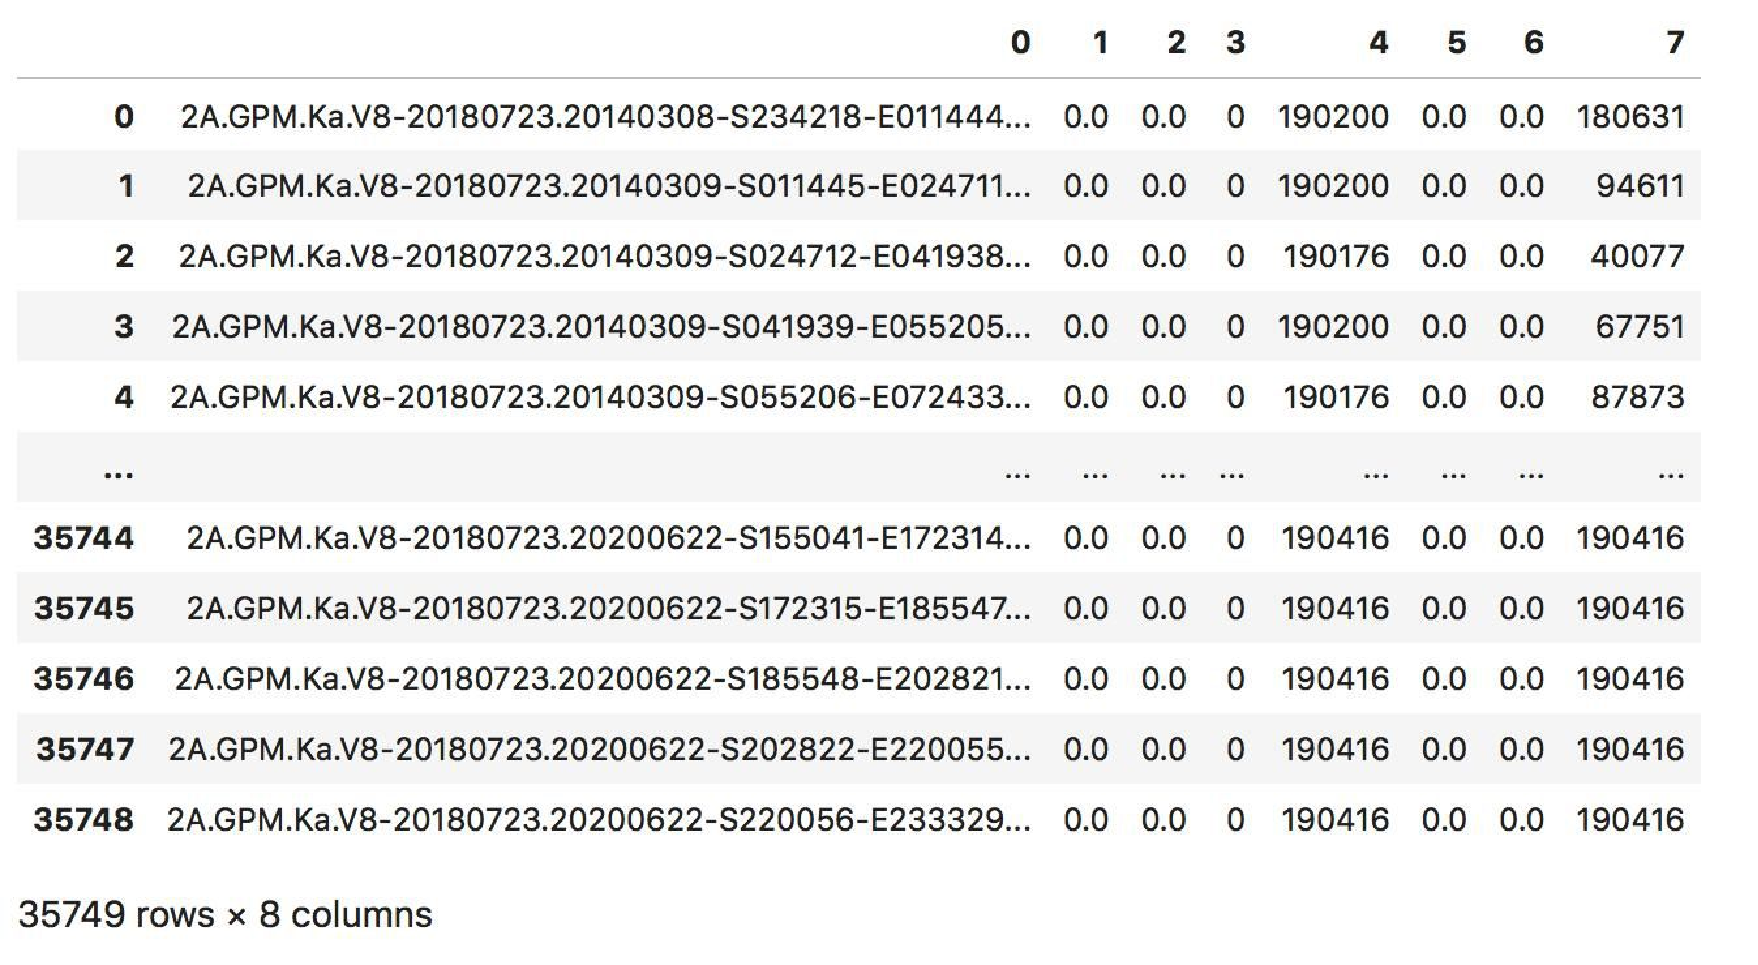
\includegraphics[width=0.8\textwidth]{weather/weather_data.pdf}
		\caption{weather data for separate coordinates.}
		\label{fig:Here we can find lot's of data and some of them are irrelevant to us. In column one we notice coordinates and date.}
	\end{center}
\end{figure}

We prepared algorithm to separate informations only for relevant ones from the first column. Now we have two coordinates separately and also the date for a measurement. 

\begin{figure}[htb]
	\begin{center}
		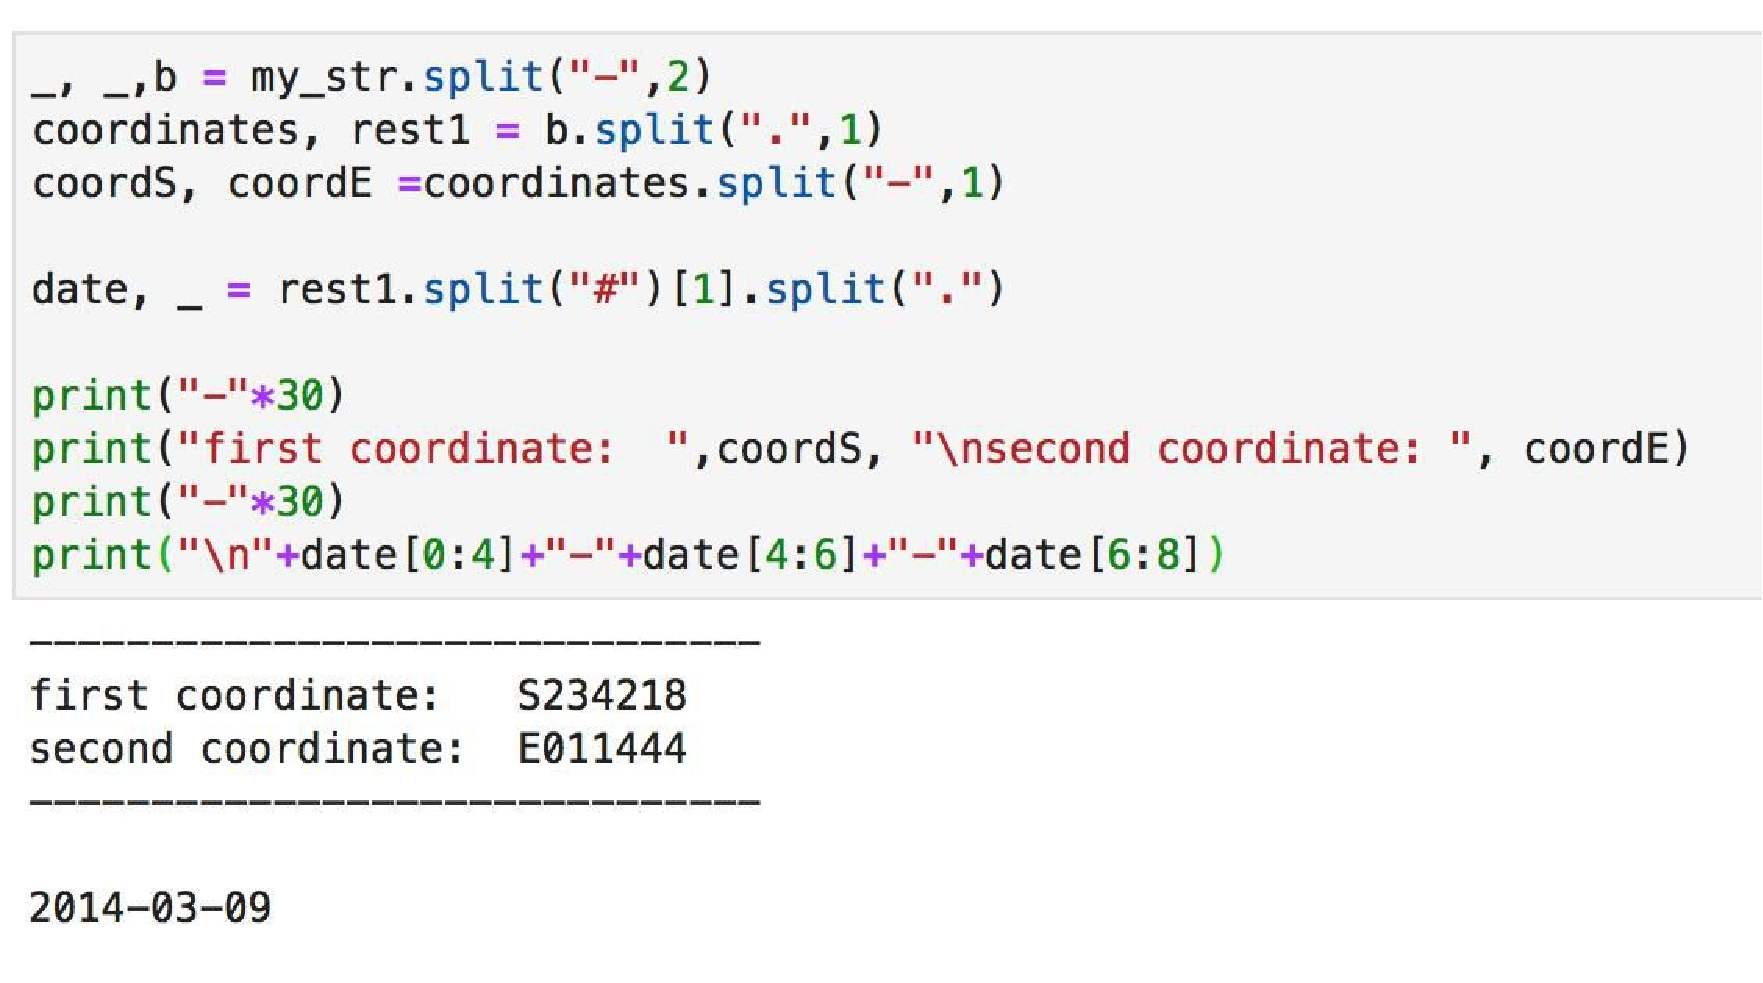
\includegraphics[width=0.8\textwidth]{weather/weather_split_data.pdf}
		\caption{Here we provide algorithm to access only relevant data from the first column such as coordinates and date. .}
		\label{fig:pSeparate coordinates and date}
	\end{center}
\end{figure}

Next step is to combine these coordinates, dates and rainfall data to show the trends. We also have knowledge how to find countries using coordinates in Python, which is very useful. The problem is that we don't know the unit of these coordinates. There are three common units - decimal degrees (DD), degrees-decimal-minutes (DDM) and degrees-minutes-seconds (DMS), but our coordinates are in different units. Also there are only coordinates for one quarter of the world (SE) and we need to find an idea how to calculate it and make it accessible to our algorithm. Since we don't know how to calculate these coordinates, we can't use it. 

